\chapter{Infravermelho}

\section*{Introdução}

\paragraph{}
No capítulo de infravermelho, iremos falar sobre o funcionamento e utilidade que os sensores infravermelhos do \textit{Sparki} possuem. As ondas infravermelhas estão mais presentes no nosso dia a dia do que você pode imaginar, na maioria das vezes elas são úteis quando utilizados receptores de luz infravermelha. Nesse capítulo iremos explicar como que o \textit{Sparki} pode ser controlado pelo controle remoto e como fazê-lo seguir linhas utilizando dessas ondas.

\section{Ondas Infravermelhas}
\paragraph{}
Para começar, que tal falarmos do que exatamente é uma onda infravermelha? Ela, assim como a luz visível, é uma onda eletromagnética, uma onda capaz de se propagar no vácuo. A luz infravermelha é invisível aos olhos humanos, isso porque nossos foto-receptores dentro dos nossos olhos, são incapazes de serem estimulados pela frequência das ondas infravermelhas.
\paragraph{}
Chamamos essa onda de infravermelho, porque a sua frequência é menor do que a frequência da cor vermelha (o prefixo infra indica que algo é inferior). A cor vermelha é a cor com a frequência mais baixa que o ser humano é capaz de enxergar, logo se temos uma onda com frequência menor, ela se torna invisível.

    \begin{figure}[h]
    \caption{Espectro da luz visível}
     
    \centering 
    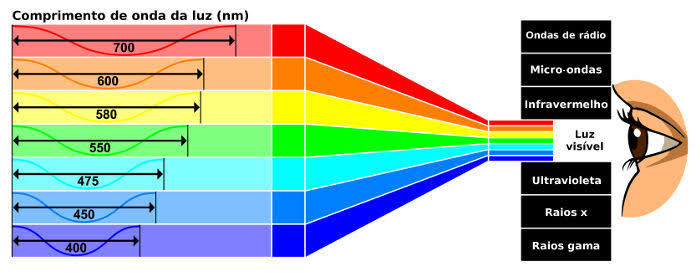
\includegraphics[width=14cm]{Figuras/espectro.jpg}
    \label{figura:espectro.jpeg}
    \end{figure}

\paragraph{}
Você deve estar lembrando do Capítulo de Ultrassom, onde falamos que ondas ultrassônicas são ondas sonoras que os seres humanos são incapazes de escutar porque possuem uma frequência muito alta, essa é a mesma lógica da luz ultravioleta, presente acima na imagem \ref{figura:espectro.jpeg}, elas são ondas eletromagnéticas com frequência mais alta do que a cor violeta, que é a cor com frequência mais alta que nós somos capazes de enxergar, logo ela também é invisível aos nossos olhos. Alguns animais são capazes de ver essas cores, logo eles conseguem ver o mundo ainda mais colorido do que nós humanos.
\paragraph{}
Os raios infravermelhos originam-se dos corpos quentes como o Sol e o corpo de seres vivos por exemplo, cada cor está relacionada com uma temperatura (se você iluminar um termômetro com luzes de cores diferentes, ele irá dar temperaturas diferentes), e o vermelho é a cor mais quente, logo mesmo sem conseguir vermos o infravermelho, ainda somos capazes de sentí-lo porque ele aquece a nossa pele.
\paragraph{}
Esse tipo de onda é muito importante para a vida na Terra, ela é responsável pelo \textbf{efeito estufa}, onde parte dos raios solares ficam presos dentro da nossa atmosfera e assim eles mantém a Terra aquecida e propensa à vida.

    \begin{figure}[h]
    \caption{Efeito estufa}
     
    \centering 
    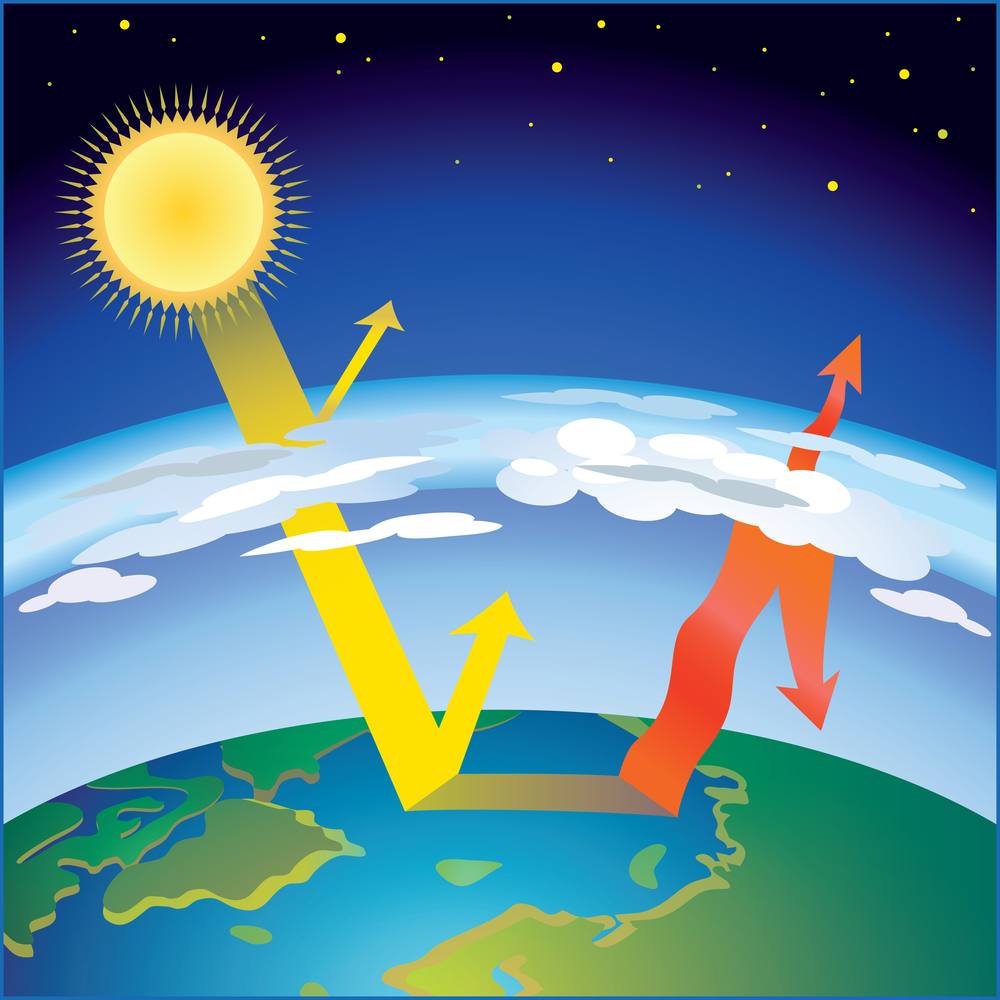
\includegraphics[width=7cm]{Figuras/estufa.jpg}
    \label{figura:estufa.jpeg}
    \end{figure}
    
\textit{Pera, pelo o que eu vi na televisão, o efeito estufa é prejudicial porque contribui para o aquecimento global, afinal ele é bom ou ruim?} \par
O que é ruim é o quanto nós humanos poluímos a atmosfera com gás carbônico. E é a presença desse gás na atmosfera que contribui para que as ondas solares fiquem presas aqui no planeta. Quanto mais jogamos ele no ar, menos as ondas são refletidas de volta para o espaço, e assim elas ficam aqui dentro nos esquentando.

\section{Aplicações no cotidiano}

\subsection{Óculos de visão noturna}
\paragraph{}
Alguns óculos de visão noturna permitem que a gente enxergue no escuro captando a radiação infravermelha do ambiente e gerando um termograma, que nada mais é do que uma imagem colorida que mostra onde está mais quente e onde está mais frio. Assim somos capazes de enxergar objetos e outras pessoas mesmo na escuridão.

\subsection{Câmeras térmicas}
\paragraph{}
Usando da mesma tecnologia que os óculos de visão noturna mencionados acima, essas câmeras convertem frequências que estão no espectro infravermelho para o espectro visível, assim conseguimos visualizar os objetos por meio do calor que eles emitem. Essas câmeras são úteis para encontrar pessoas ou animais em meio a vegetação, destroços ou esconderijos, além de poder encontrar falhas em equipamentos dependendo de onde estiver mais quente ou mais frio do que o normal.

\subsection{Controles remotos}
\paragraph{}
Quando você aperta um botão do seu controle remoto para mudar o canal da sua televisão, ele se comunica com a TV utilizando dos raios infravermelhos, se você apontar a câmera do seu celular para a lampadazinha na ponta do seu controle e apertar algum botão, você conseguirá enxergar os raios sendo emitidos. A seguir iremos explicar como que essa comunicação funciona.

\section{Controle infravermelho}
\label{ref:controle}
\paragraph{}
Agora vamos começar a falar sobre como podemos controlar o \textit{Sparki} utilizando o controle remoto, que vem junto com o kit. Ele funciona emitindo luz infravermelha a partir de sua lâmpada, luz essa que deve ser captada pelo sensor de infravermelho presente no \textit{Sparki}.

    \begin{figure}[h]
    \caption{Sensor de infravermelho}
     
    \centering 
    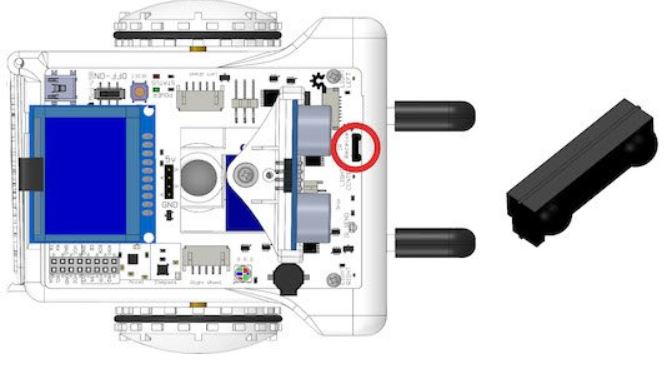
\includegraphics[width=7cm]{Figuras/sensor.JPG}
    \label{figura:sensor.jpeg}
    \end{figure}

\paragraph{}
Cada botão do controle remoto possui um padrão a ele relacionado, esse padrão representa quantas vezes a lâmpada do controle deve piscar e por quanto tempo, o sensor recebe esse padrão e o \textit{Sparki} é responsável por traduzir esse padrão para o botão correspondente. Para ficar mais fácil de entender é só lembrarmos do código Morse, onde cada letra e número é associado a um conjunto de pontos e traços. O que o controle remoto faz é parecido com a tradução de uma palavra em português  para código Morse, e depois o nosso robô deve saber ler essa palavra em código Morse e traduzir de volta para o português.

    \begin{center}
    \textcolor{mydarkblue}{\textbf{Atençao!}}
    \\ Os sinais infravermelhos não estão em código Morse, mencionamos ele apenas como forma de facilitar a compreensão. No geral, controles remotos têm padrões diferentes um do outro.
    \end{center}

\paragraph{}
Para facilitar a nossa vida, os criadores do \textit{Sparki} atribuíram a cada botão um número inteiro, como pode ser observado na Figura 8.4.

    \begin{figure}[h]
    \caption{Mapeamentos do controle}
     
    \centering 
    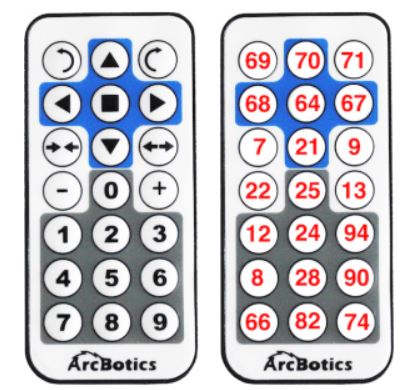
\includegraphics[width=5cm]{Figuras/controle.JPG}
    \label{figura:controle.jpeg}
    \end{figure}
    
\paragraph{}
Assim, quando utilizamos a função \lstinline[columns=fixed]{sparki.readIR()}, ela retorna o número inteiro associado ao botão que foi apertado. Para obtermos algum comando do controle devemos ter como base o seguinte código:

    \begin{lstlisting}[language=C]
#include <Sparki.h>;

int botao;

void setup()
{
}

void loop()
{
    botao = sparki.readIR();
}
\end{lstlisting}
    
Esta função salva na nossa variável inteira o número correspondente ao último botão que foi apertado antes dela ser chamada, caso não tenhamos apertado nenhum botão, ela irá salvar o valor \"-1".

\paragraph{}
Graças ao capítulo de \textit{if e else}, podemos escrever um algoritmo que executa uma atividade diferente para cada botão que for apertado, podemos controlar a movimentação do nosso robô da seguinte forma, por exemplo:

    \begin{lstlisting}[language=C]
#include <Sparki.h>;

int botao;

void setup()
{
}

void loop()
{
    botao = sparki.readIR();
    if(botao == 70)
    {
        sparki.moveStop();
        sparki.moveForward();
    }
    else if(botao == 67)
    {
        sparki.moveStop();
        sparki.moveRight();
    }
    else if(botao == 68)
    {
        sparki.moveStop();
        sparki.moveLeft();
    }
    else if(botao == 21)
    {
        sparki.moveStop();
        sparki.moveBackward();
    }
    else if(botao == 64)
    {
        sparki.moveStop();
    }
    delay(1000);
}
\end{lstlisting}

\section{Vetor de sensores infravermelhos}

\paragraph{}
Talvez você nunca tenha reparado, mas embaixo do \textit{Sparki} possui cinco retângulos pretos perto da garra, três no meio e um em cada canto. Esses retângulos são nada mais nada menos do que os sensores infravermelhos responsáveis por medir a \textbf{reflectância} da luz do chão abaixo dele (a reflectância de um corpo é a quantidade de luz que ele reflete).

\begin{comment}
Criar um card ilustrando o conceito de reflectância 
\end{comment}

    \begin{figure}[h]
    \caption{Os cinco sensores de reflectância infravermelha}
     
    \centering 
    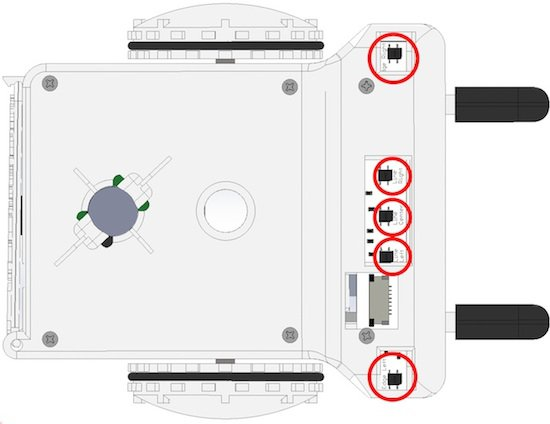
\includegraphics[width=8cm]{Figuras/vetor.jpg}
    \label{figura:vetor.jpeg}
    \end{figure}

\paragraph{}
Você já deve ter ouvido falar que a cor preta é a ausência de todas as cores, enquanto o branco é quando todas elas estão presentes, isso porque uma superfície preta absorve todas as frequências do espectro visível, enquanto o branco reflete todas de volta. Já uma superfície amarela, por exemplo, absorve todas as frequências menos a do amarelo, por isso vemos ela da cor amarela, porque foi a única frequência refletida para os nossos olhos. Como você já deve ter percebido, quando medimos a reflectância de uma superfície branca, certamente o valor será bem maior do que a de uma superfície preta.
\\~\\
\textit{Esses sensores então são utilizados para conseguirmos identificar quais são as cores que estão embaixo do Sparki?} \par
Essa é uma questão interessante! É sim possível diferenciar algumas cores pela sua reflectância. Mas até mesmo cores bem diferentes podem representar valores iguais ou muito semelhantes, e os sensores não são tão precisos e adequados para essa situação, certamente haverão muitos enganos. A verdadeira utilização deles é conseguir diferenciar superfícies mais escuras das mais claras, e isso é de extrema importância quando queremos fazer um exercício muito importante, um robô segue linhas, que normalmente anda por cima das linhas pretas num fundo branco.

\paragraph{}
É necessário certo cuidado ao utilizar esses sensores, porque uma mesma superfície pode retornar valores diferentes de reflectância, não podemos garantir que esteja tudo pintado no exato mesmo tom ou que haja a mesma incidência de luz em todo lugar, por isso quando mexemos com valores de reflectância devemos adotar \textbf{limiares}. Limiares são intervalos de valores que, embora diferentes um do outro, consideramos como sendo a mesma coisa, daremos como exemplo a separação das fases da vida, temos a fase infantil, adulta e terceira idade por exemplo, e dependendo da sua idade você irá se encaixar em uma dessas três fases.
\\~\\
\begin{tabular}{|c|c|c|c|c|c|}
    \cline{1-6}
     Limiares & 0 a 1 ano & 1 a 12 anos & 12 a 18 anos & 18 a 60 anos & 60 anos em diante \\
     \hline
     Classificação & Bebê & Criança & Adolescente & Adulto & Idoso \\
     \hline
\end{tabular}

\paragraph{}
A quantidade de limiares que vamos utilizar depende do problema do qual estamos tratando, na situação acima talvez fosse conveniente utilizar apenas 5 limiares, mas pode ser que em outra situação você teria que passar a incluir classificações como pré-adolescente ou ancião. Depois de determinados quais serão nossos limiares, podemos começar a coletar dados e então separá-los e classificá-los. Por exemplo, você tem 16 anos? Então você é um adolescente. Você tem 20 anos? Então você é um adulto. Você tem 14 anos, 7 meses, 2 semanas, 5 dias, 14 horas e meia de vida? Então você é considerado como sendo um adolescente também.

\paragraph{}
A importância do exemplo acima é fazer você entender que mais de um valor pode significar a mesma coisa, porque ao utilizar os sensores infravermelhos, você irá receber muitos valores de reflectância diferentes um do outro, e mesmo assim todos eles querem dizer que o chão é preto ou não, ou quem sabe só um pouco claro.

\subsection{Função}
\paragraph{}
Enfim, já está na hora de ensinarmos como você recebe esses valores de reflectância não é mesmo? Para cada um dos 5 sensores, existe uma função diferente que o ativa, ela nos retorna então um número \textbf{inteiro}, o qual devemos salvar numa variável inteira. As funções que ativam os sensores são: \lstinline[columns=fixed]{sparki.lineLeft()},\lstinline[columns=fixed]{sparki.lineRight()}, \lstinline[columns=fixed]{sparki.lineCenter()}, \lstinline[columns=fixed]{sparki.edgeLeft()} e \lstinline[columns=fixed]{sparki.edgeRight()}.

    \begin{center}
    \textcolor{mydarkblue}{\textbf{Para não esquecer!}}
    \\``Left'' traduzido para o português significa ``Esquerda'', ``Right'' significa ``Direita'' e ``Edge'' significa ``Borda ou Beira''.
    \end{center}
    
\paragraph{}
Caso estejamos interessados em saber se o \textit{Sparki} está pisando em cima de uma linha ou não, podemos escrever o seguinte código (vamos considerar que uma reflectância abaixo de 300 significa que a cor é preta e que acima disso a cor é branca).

    \begin{lstlisting}[language=C]
#include <Sparki.h>;

int limiar = 300, esquerda, centro, direita;

void setup()
{
sparki.clearLCD();
sparki.updateLCD();
}

void loop()
{
    esquerda = sparki.lineLeft();
    centro   = sparki.lineCenter();
    direita  = sparki.lineRight();
    delay(500);
if(esquerda < limiar || centro < limiar || direita < limiar)
{
    sparki.clearLCD();
    sparki.print("O Sparki está em cima de uma linha");
    sparki.updateLCD();
} else
{
    sparki.clearLCD();
    sparki.print("O Sparki NÃO está em cima de uma linha");
    sparki.updateLCD();
}
delay(500);
}
\end{lstlisting}

Nesse caso, se qualquer um dos 3 sensores do meio identificar a cor preta, estamos assumindo que o \textit{Sparki} está passando em cima de uma linha.
\\~\\
\textit{Calma lá! Mas afinal, por que esses sensores se chamam sensores infravermelhos? O que eles tem a ver com a luz infravermelha?} \par
Opa, desculpa! A razão do nome é porque junto com esses sensores, de baixo do \textit{Sparki}, nós temos LEDs (diodos emissores de luz) que emitem raios infravermelhos que serão refletidos pelo chão, e são esses raios que os sensores irão utilizar para medir a reflectância do chão.

\section{Exercícios}

    \question{Queremos que o \textit{Sparki} ande, pegue algum objeto com a sua garra e depois largue-o em algum outro lugar, escreva um algoritmo que permita que a gente, utilizando apenas o controle remoto, consiga fazer essa tarefa (se quiser você pode começar usando o código presente na seção \ref{ref:controle}). Suponha que a garra esteja inicialmente aberta.}

    \begin{center}
        \line(1,0){450}
        \vspace{0.2cm}   
        \line(1,0){450}
        \vspace{0.2cm}   
        \line(1,0){450}
        \vspace{0.2cm}   
        \line(1,0){450}
        \vspace{0.2cm}   
        \line(1,0){450}
        \vspace{0.4cm} 
    \end{center}

    \question{Escreva um código que faça com que o \textit{Sparki} faça contas de adição e de subtração com os números de 0 a 3 e que mostre o resultado da conta na tela LCD. Os números e a operação devem ser escolhidos apertando os botões do controle remoto.}
    
    \begin{center}
        \line(1,0){450}
        \vspace{0.2cm}   
        \line(1,0){450}
        \vspace{0.2cm}   
        \line(1,0){450}
        \vspace{0.2cm}   
        \line(1,0){450}
        \vspace{0.2cm}   
        \line(1,0){450}
        \vspace{0.4cm} 
    \end{center}

    \question{Escreva um código onde o \textit{Sparki} anda 5 centímetros em linha reta enquanto vai medindo a reflectância da superfície abaixo dele a cada centímetro e então calcula a reflectância média da superfície utilizando média aritmética.}
    
    \begin{center}
        \line(1,0){450}
        \vspace{0.2cm}   
        \line(1,0){450}
        \vspace{0.2cm}   
        \line(1,0){450}
        \vspace{0.2cm}   
        \line(1,0){450}
        \vspace{0.2cm}   
        \line(1,0){450}
        \vspace{0.4cm} 
    \end{center}

    \question{Utilizando dos sensores de reflectância infravermelha das bordas e o do centro, faça um programa onde o \textit{Sparki} ande em linha reta em cima de uma mesa e então PARE quando ele identificar que vai cair da mesa. Suponha que a mesa inteira seja da mesma cor e que quando a reflectância for menos do que 200, então passamos dos limites da mesa.}

    \begin{center}
        \line(1,0){450}
        \vspace{0.2cm}   
        \line(1,0){450}
        \vspace{0.2cm}   
        \line(1,0){450}
        \vspace{0.2cm}   
        \line(1,0){450}
        \vspace{0.2cm}   
        \line(1,0){450}
        \vspace{0.4cm} 
    \end{center}

    \challenge{\large{Desafio: escreva um programa onde o \textit{Sparki} seja capaz de andar por cima da faixa preta do percurso representado abaixo, fazendo com que ele fique andando em círculos (ele deve começar do traço no canto esquerdo inferior).}}

    \begin{figure}[h]
     
    \centering 
        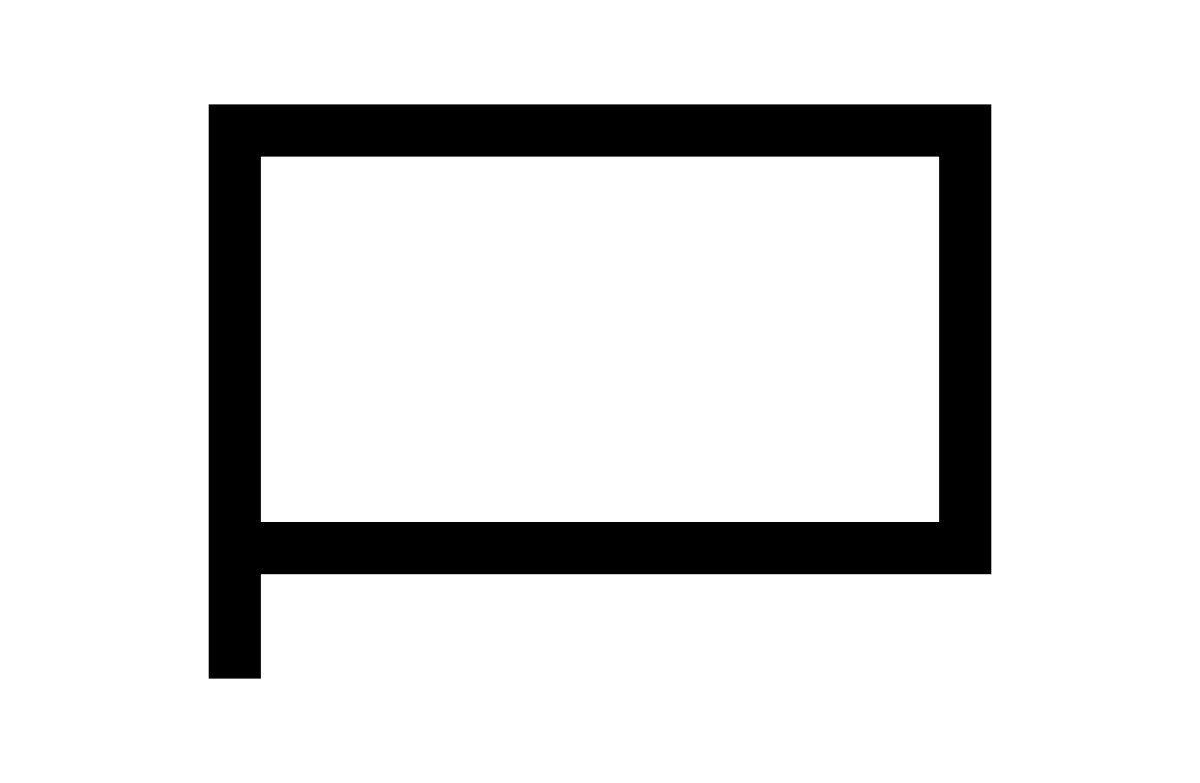
\includegraphics[width=5cm]{Figuras/trajeto.png}
        \label{figura:trajeto.jpeg}
    \end{figure}
    
    \begin{center}
        \line(1,0){450}
        \vspace{0.2cm}   
        \line(1,0){450}
        \vspace{0.2cm}   
        \line(1,0){450}
        \vspace{0.2cm}   
        \line(1,0){450}
        \vspace{0.2cm}   
        \line(1,0){450}
        \vspace{0.4cm} 
    \end{center}